\chapter{Benchmarking and Result}

\section{Fine Tuning the Deep Learning Models}

On top of the five main dataset of size $> 20k$, DeepPrime has additional 18 datasets of size $\sim5k$, which were used to fine tune the model for better generalizability. As a result, for a more thorough comparison between the models, the same fine tuning process was conducted on all deep learning models.

To fine tune the models, the same hyperparameters were used as the original training, except for the learning rate, which was set to $1e-3$ for the fine tuning to accommodate the smaller dataset size. The sequence processing layers were frozen, leaving only the feature processing and the final meta learner to be trained. The models were trained for at most 300 epochs for each fold, and the best model was selected based on the validation loss.

\section{Benchmarking}

To test how the different models compare on a variety of datasets, 

% TODO: add references to the section and appendix after including the results
As mentioned in section {ensemble training}, although both PRIDICT and DeepPrime uses different features, for a more direct comparison of the architecture, both models were retrained using the features selected from this study.

\subsection{Performance on All Datasets}

As discussed in \autoref{sec:ensemble}, all three ensemble models were able to significantly outperform the base learners on the PRIDICT HEK293T PE2 dataset. Thus, power weighted mean ensemble, bagging and adaboost were trained on all available datasets alongside the transformer model to evaluate their performance against the base learners, as well as DeepPrime and PRIDICT.



\section{Attention Analysis}
\label{sec:attention_analysis}

\begin{figure}
    \centering
    \subfigure[Substitution]{
        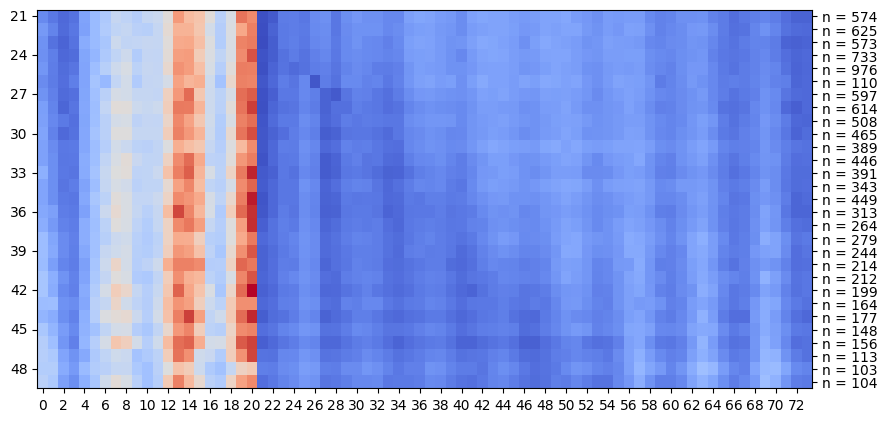
\includegraphics[width=0.88\textwidth]{dp-hek293t-pe2-transformer-only-attention-insertion.png}
        \label{fig:attention_insertion}
    }
    \subfigure[Insertion]{
        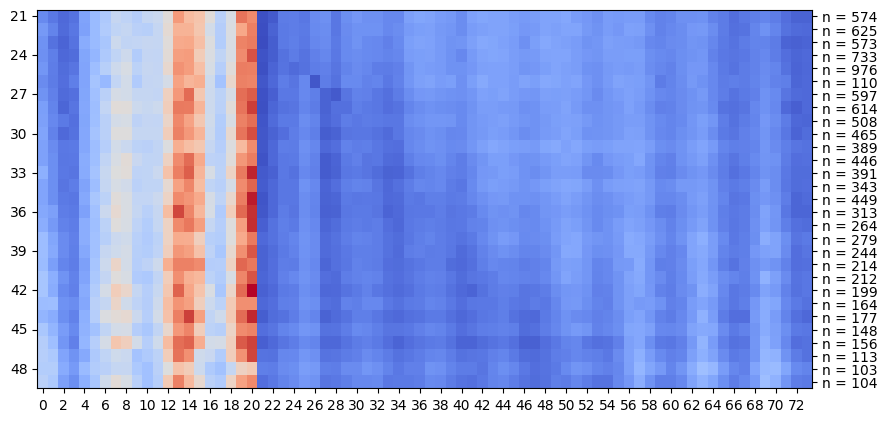
\includegraphics[width=0.88\textwidth]{dp-hek293t-pe2-transformer-only-attention-insertion.png}
        \label{fig:attention_substitution}
    }
    \subfigure[Deletion]{
        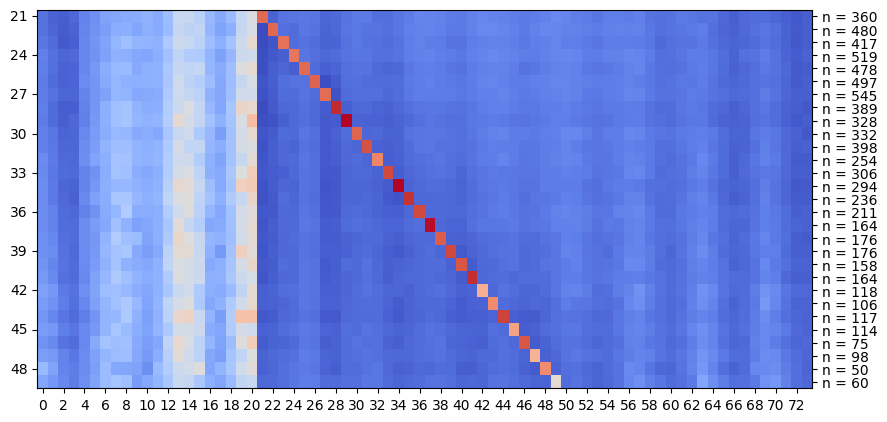
\includegraphics[width=0.88\textwidth]{dp-hek293t-pe2-transformer-only-attention-deletion.png}
        \label{fig:attention_deletion}
    }
    \caption[Attention weights for the DeepPrime model trained on the HEK293T-PE2 dataset]{Attention weights of length 1 edits for the DeepPrime model trained on the HEK293T-PE2 dataset. The x-axis represents the position of the transformer output token, the y-axis indicates the edit position. Red colour indicates higher attention weights, while blue indicates lower attention weights. The example size for each edit location is shown on the right in the format of 'n=number of examples'.}
    \label{fig:attention}
\end{figure}

A significant advantage of the attention based methods are their interpretability. The attention mechanism allows the model to focus on specific parts of the input data using the attention weights, which can be visualized teo understand the model's decision making process. 

In this architecture, the most informative and interpretable attention weights are the feature embedding attention weights at the final layer of the transformer model, pooling all token embeddings into a single feature embedding. 

The examples were grouped together by their editing type and length so that the edit positions can be easily identified and compared. And the attention weights for edits at the same position were aggregated to show the overall importance of the position in the editing efficiency prediction.

The model trained on the biggest DeepPrime dataset was first tested, as the transformer model has the greatest chance of learning the underlying motifs influencing the editing efficiency in the data. Starting with the edits of length 1, the attention weights were visualized for the substitution, insertion, and deletion, shown in \autoref{fig:attention}. 

For both 1-bp substitution and insertion, the attention weights were the highest from around the start of the protospacer location (location 4) to the nick position (location 20, also where the PBS ends). This may be an indication that the model considers the composition of the PBS as an important feature for the editing efficiency prediction. Additionally, one of the hot spots for the attention weights was the protospacer location 13 to 17. This is consistent with the finding in \autoref{fig:shap} that the composition of the protospacer is an important feature for the editing efficiency prediction.

However, for deletion, the attention weights were the highest at the edit position. The cross attention output of the edit position for deletion was dominated by the encoder output, as the self-attention weights for the mutated sequence at edit position were masked out to be zero. This is a possible indication that the model considers the base to delete as an important feature for the deletion operation.

\begin{figure}
    \centering
    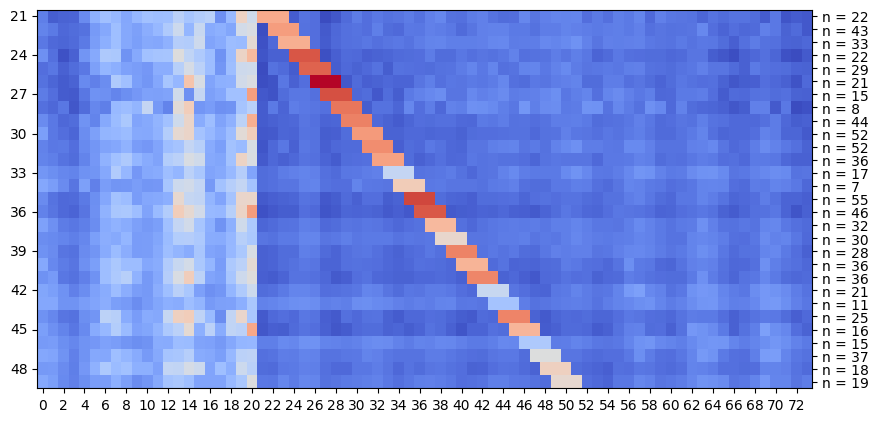
\includegraphics[width=0.9\textwidth]{dp-hek293t-pe2-transformer-only-attention-deletion-3bp.png}
    \caption[Attention weights for 3-bp deletion of the DeepPrime model trained on the HEK293T-PE2 dataset]{Similar to \autoref{fig:attention}, attention weights of length 3 deletion for the DeepPrime model trained on the HEK293T-PE2 dataset.}
    \label{fig:attention_deletion_3bp}
\end{figure}

The attention weights for the edits of length 3 showed similar result (\autoref{fig:attention_deletion_3bp}), the only noticeable difference is that the high attention regions for deletion were extended to 3bp long, reflecting the longer deletion length.

During SHAP analysis in \autoref{sec:determinants}, the edited base was not investigated, as a meaningful representation for bases of different lengths could not be found. Thus, to understand if the base to edit during deletion is indeed an important feature, SHAP analysis was conducted again on the HEK293T PE2 